\section{Задание}

Запросы к серверу бывают двух типов: запросы к любому АПИ или запросы, которые определяют использование старого АПИ. Новый АПИ вернется к старому АПИ, если новый сервер занят.
Если все три имеющихся оператора заняты, запросу отказывают в обслуживании.

Генератор, который генерирует запросы любого типа, и тот, который генерирует только запросы к старому АПИ, имеет время для обработки запроса, следуя распределению $U(10,15)$ и $U(10,18)$ соответственно.
Три оператора имеют разную производительность, время обработки запроса которых соответствует правилам $U(10,20), U(20,25), U(15,30)$.
Четыре компьютера, время обработки запроса которых соответствует правилам $N(20,4^2), N(30,5^2), N(20,4^2), N(30,5^2)$.

Промоделировать процесс обработки 500 запросов.

\section{Теоритическая часть}

Необходимо создать концептуальную модель в терминах СМО, определить эндогенные и экзогенные переменные.
За единицу системного времени выбрать 0,01 минуты.

\begin{figure}[h!]
\centering
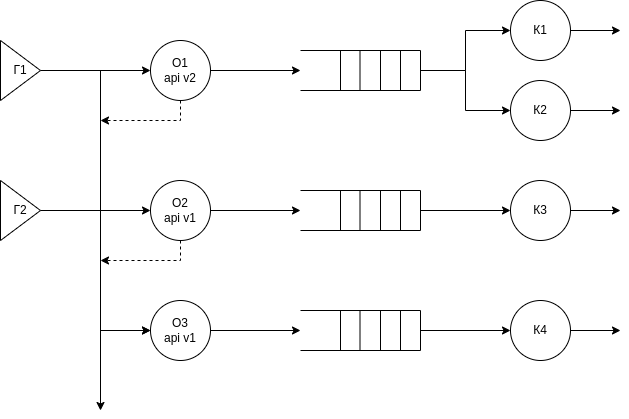
\includegraphics[width=0.8\textwidth]{6/6_system}
\end{figure}


В процессе взаимодействия клиентов с информационным центром возможно:

\begin{itemize}
    \item Режим нормального обслуживания, т.е. клиент выбирает одного из свободных операторов, отдавая предпочтение тому у которого меньше номер.
    \item Режим отказа в обслуживании клиента, когда все операторы заняты
\end{itemize}

Переменные и уравнения имитационной модели.

\begin{itemize}
    \item Эндогенные переменные: время обработки задания i-ым оператором, время решения этого задания j-ым компьютером.
    \item Экзогенные переменные: число обслуженных клиентов и число клиентов получивших отказ.
\end{itemize}


Вероятность отказа:
\begin{equation*}
    P_{\text{отк}} = \frac{C_{\text{отк}}}{C_{\text{отк}} + C_{\text{обсл}}}
\end{equation*}

\section{Результаты}

\begin{figure}[h!]
    \centering
    \fbox{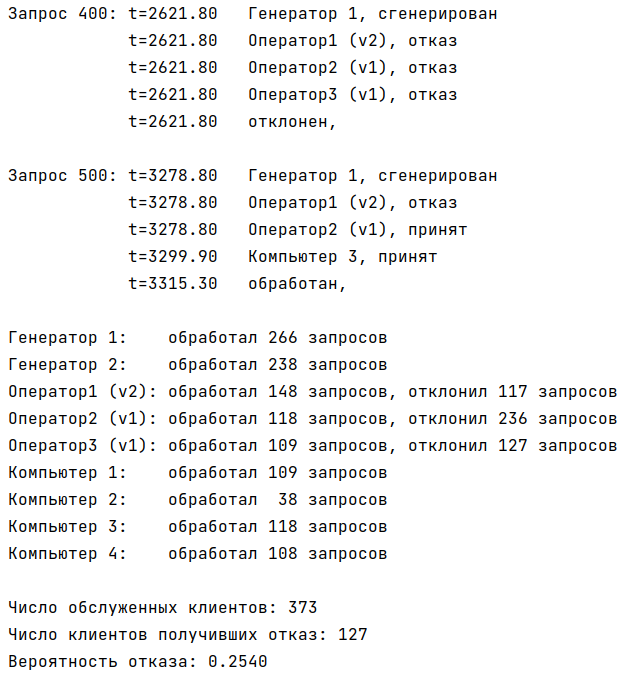
\includegraphics[width=0.8\textwidth]{6/ex}}
\end{figure}

\pagebreak
\section{Листинг кода}

% \onehalfspacing

\lstinputlisting[language=Python, caption=Программная реализация информационного центра]{../6/main.py}

\pagebreak
\setstretch{1.16}
\lstinputlisting[language=Python, caption=Программный интерфейс]{../6/system/model.py}
